\documentclass{beamer}
%\usepackage[margin=1in]{geometry}
\usepackage{amsthm,amsmath,amsfonts,hyperref,graphicx,color,multicol}
\usepackage{enumitem,tikz}

%%%%%%%%%%
%Beamer Template Customization
%%%%%%%%%%
\setbeamertemplate{navigation symbols}{}
\setbeamertemplate{theorems}[ams style]
\setbeamertemplate{blocks}[rounded]

\definecolor{Blu}{RGB}{43,62,133} % UWEC Blue
\setbeamercolor{structure}{fg=Blu} % Titles

%Unnumbered footnotes:
\newcommand{\blfootnote}[1]{%
	\begingroup
	\renewcommand\thefootnote{}\footnote{#1}%
	\addtocounter{footnote}{-1}%
	\endgroup
}


%%%%%%%%%%
%Custom Commands
%%%%%%%%%%
\newcommand{\R}{\mathbb{R}}
\newcommand{\veca}{\vec{a}}
\newcommand{\vecb}{\vec{b}}
\newcommand{\vece}{\vec{e}}
\newcommand{\vecu}{\vec{u}}
\newcommand{\vecv}{\vec{v}}
\newcommand{\vecw}{\vec{w}}
\newcommand{\vecx}{\vec{x}}
\newcommand{\zerovector}{\vec{0}}

\newcommand{\ds}{\displaystyle}

\newcommand{\fn}{\insertframenumber}

\newcommand{\col}{\operatorname{col}}
\newcommand{\row}{\operatorname{row}}
\newcommand{\rank}{\operatorname{rank}}
\newcommand{\adj}{\operatorname{adj}}

\newcommand{\blank}[1]{\underline{\hspace*{#1}}}


%%%%%%%%%%
%Custom Theorem Environments
%%%%%%%%%%
\theoremstyle{definition}
\newtheorem{exercise}{Exercise}
\newtheorem{question}[exercise]{Question}
\newtheorem*{defn}{Definition}
\newtheorem*{exa}{Example}
\newtheorem*{disc}{Group Discussion}
\newtheorem*{nb}{Note}
\newtheorem*{recall}{Recall}
\renewcommand{\emph}[1]{{\color{blue}\texttt{#1}}}

\definecolor{Gold}{RGB}{237, 172, 26}
%Statement block
\newenvironment{statementblock}[1]{%
	\setbeamercolor{block body}{bg=Gold!20}
	\setbeamercolor{block title}{bg=Gold}
	\begin{block}{\textbf{#1.}}}{\end{block}}





\begin{document}
	\title{Math 324: Linear Algebra}
	\subtitle{Section 4.6: Row and Column Spaces}
	\author{Mckenzie West}
	\date{Last Updated: \today}
\begin{frame}
\maketitle
\end{frame}

\begin{frame}{\insertframenumber}
	\begin{block}{\textbf{Last Time.}}
	\begin{itemize}[label=--]
		\item Dimension
	\end{itemize}
	\end{block}
	\begin{block}{\textbf{Today.}}
		\begin{itemize}[label=--]
			\item Row and Column Spaces
			\item Rank of a Matrix
		\end{itemize}
	\end{block}
\end{frame}
\begin{frame}{\fn}
	\begin{exercise}[review of section 4.5]
		Consider the subspace of $\R^4\underline{}$, given by
			\[W=\left\{(a,b,a,b)\ :\ a,b\in\R\right\}.\]
		\begin{enumerate}[label=(\alph*)]
			\item Find a basis for $W$.
			\item Determine the dimension of $W$.
		\end{enumerate}
	\end{exercise}
\end{frame}
\begin{frame}{\fn}
	\begin{defn}
		Let $A$ be an $m\times n$ matrix.
		\begin{enumerate}[label=\textbf{\arabic*.}]
			\item The \emph{column space} of $A$, denoted $\col(A)$, is the subspace of $\R^m$ that is spanned by the columns of $A$.
			\item the \emph{row space} of $A$, denoted $\row(A)$, is the subspace of $\R^n$ that is spanned by the rows of $A$.
		\end{enumerate}
	\end{defn}
	\begin{exa}
		For $A=\begin{bmatrix}
			8 & -1 & 7 & 0 \\
			0 & -1 & -1 & 3 \\
			0 & -3 & -3 & 9
			\end{bmatrix}$,
		\begin{itemize}[label=--]
			\item $\col(A)$ is a subspace of $\R^3$ because each column has 3 entries
			\item  $\row(A)$ is a subspace of $\R^4$ because each row has 4 entries
		\end{itemize}
	\end{exa}
\end{frame}
\begin{frame}{\fn}
	\begin{statementblock}{Theorem 4.13}
		If an $m\times n$ matrix $A$ is row-equivalent to an $m\times n$ matrix $B$, then $\row(A)=\row(B)$.
	\end{statementblock}
	\begin{statementblock}{Theorem 4.14}
	If a matrix $A$ is row-equivalent to a $B$ that is in row-echelon form, then the non-zero rows of $B$ form a basis for $\row(A)$.
	\end{statementblock}
	\begin{exercise}
		Let $A=\begin{bmatrix}
		8 & -1 & 7 & 0 \\
		0 & -1 & -1 & 3 \\
		0 & -3 & -3 & 9
		\end{bmatrix}$.
		
		 Find a basis for $\row(A)$.  What is the dimension of $\row(A)$?
	\end{exercise}
\end{frame}
\begin{frame}{\fn}
	\begin{exercise}
		Let $A=\begin{bmatrix}
		8 & -1 & 7 & 0 \\
		0 & -1 & -1 & 3 \\
		0 & -3 & -3 & 9
		\end{bmatrix}$.
		
		Consider the matrix $A^T$. 
		\begin{enumerate}[label=(\alph*)]
			\item Convince yourself that $\col(A)=\row(A^T)$.
			\item Find a basis for $\row(A^T)$ using Theorem 4.14.
			\item What is a basis for and the dimension of $\col(A)$?
		\end{enumerate}
	\end{exercise}
\end{frame}
\begin{frame}{\fn}
\begin{exercise}
	Find a basis for $\col(A)$ and $\row(A)$ for 
	\[A=\begin{bmatrix}
	5 & 1 & -9 & -5 & 2 \\
	2 & 8 & 4 & -2 & 9 \\
	3 & -5 & -11 & -3 & -3 \\
	-3 & 2 & 8 & 3 & 7
	\end{bmatrix}\]
\end{exercise}
\end{frame}
\begin{frame}{\fn}
\begin{exercise}
	Find a basis for $\col(A)$ and $\row(A)$ for 
	\[A=\begin{bmatrix}
	7 & -5 \\
	2 & 7 \\
	-2 & 3 \\
	9 & 9
	\end{bmatrix}\]
\end{exercise}
\end{frame}
\begin{frame}{\fn}
	\begin{block}{\textbf{Brain Break.}}
		What one non-essential item do you wish you had more of?
		\begin{center}
			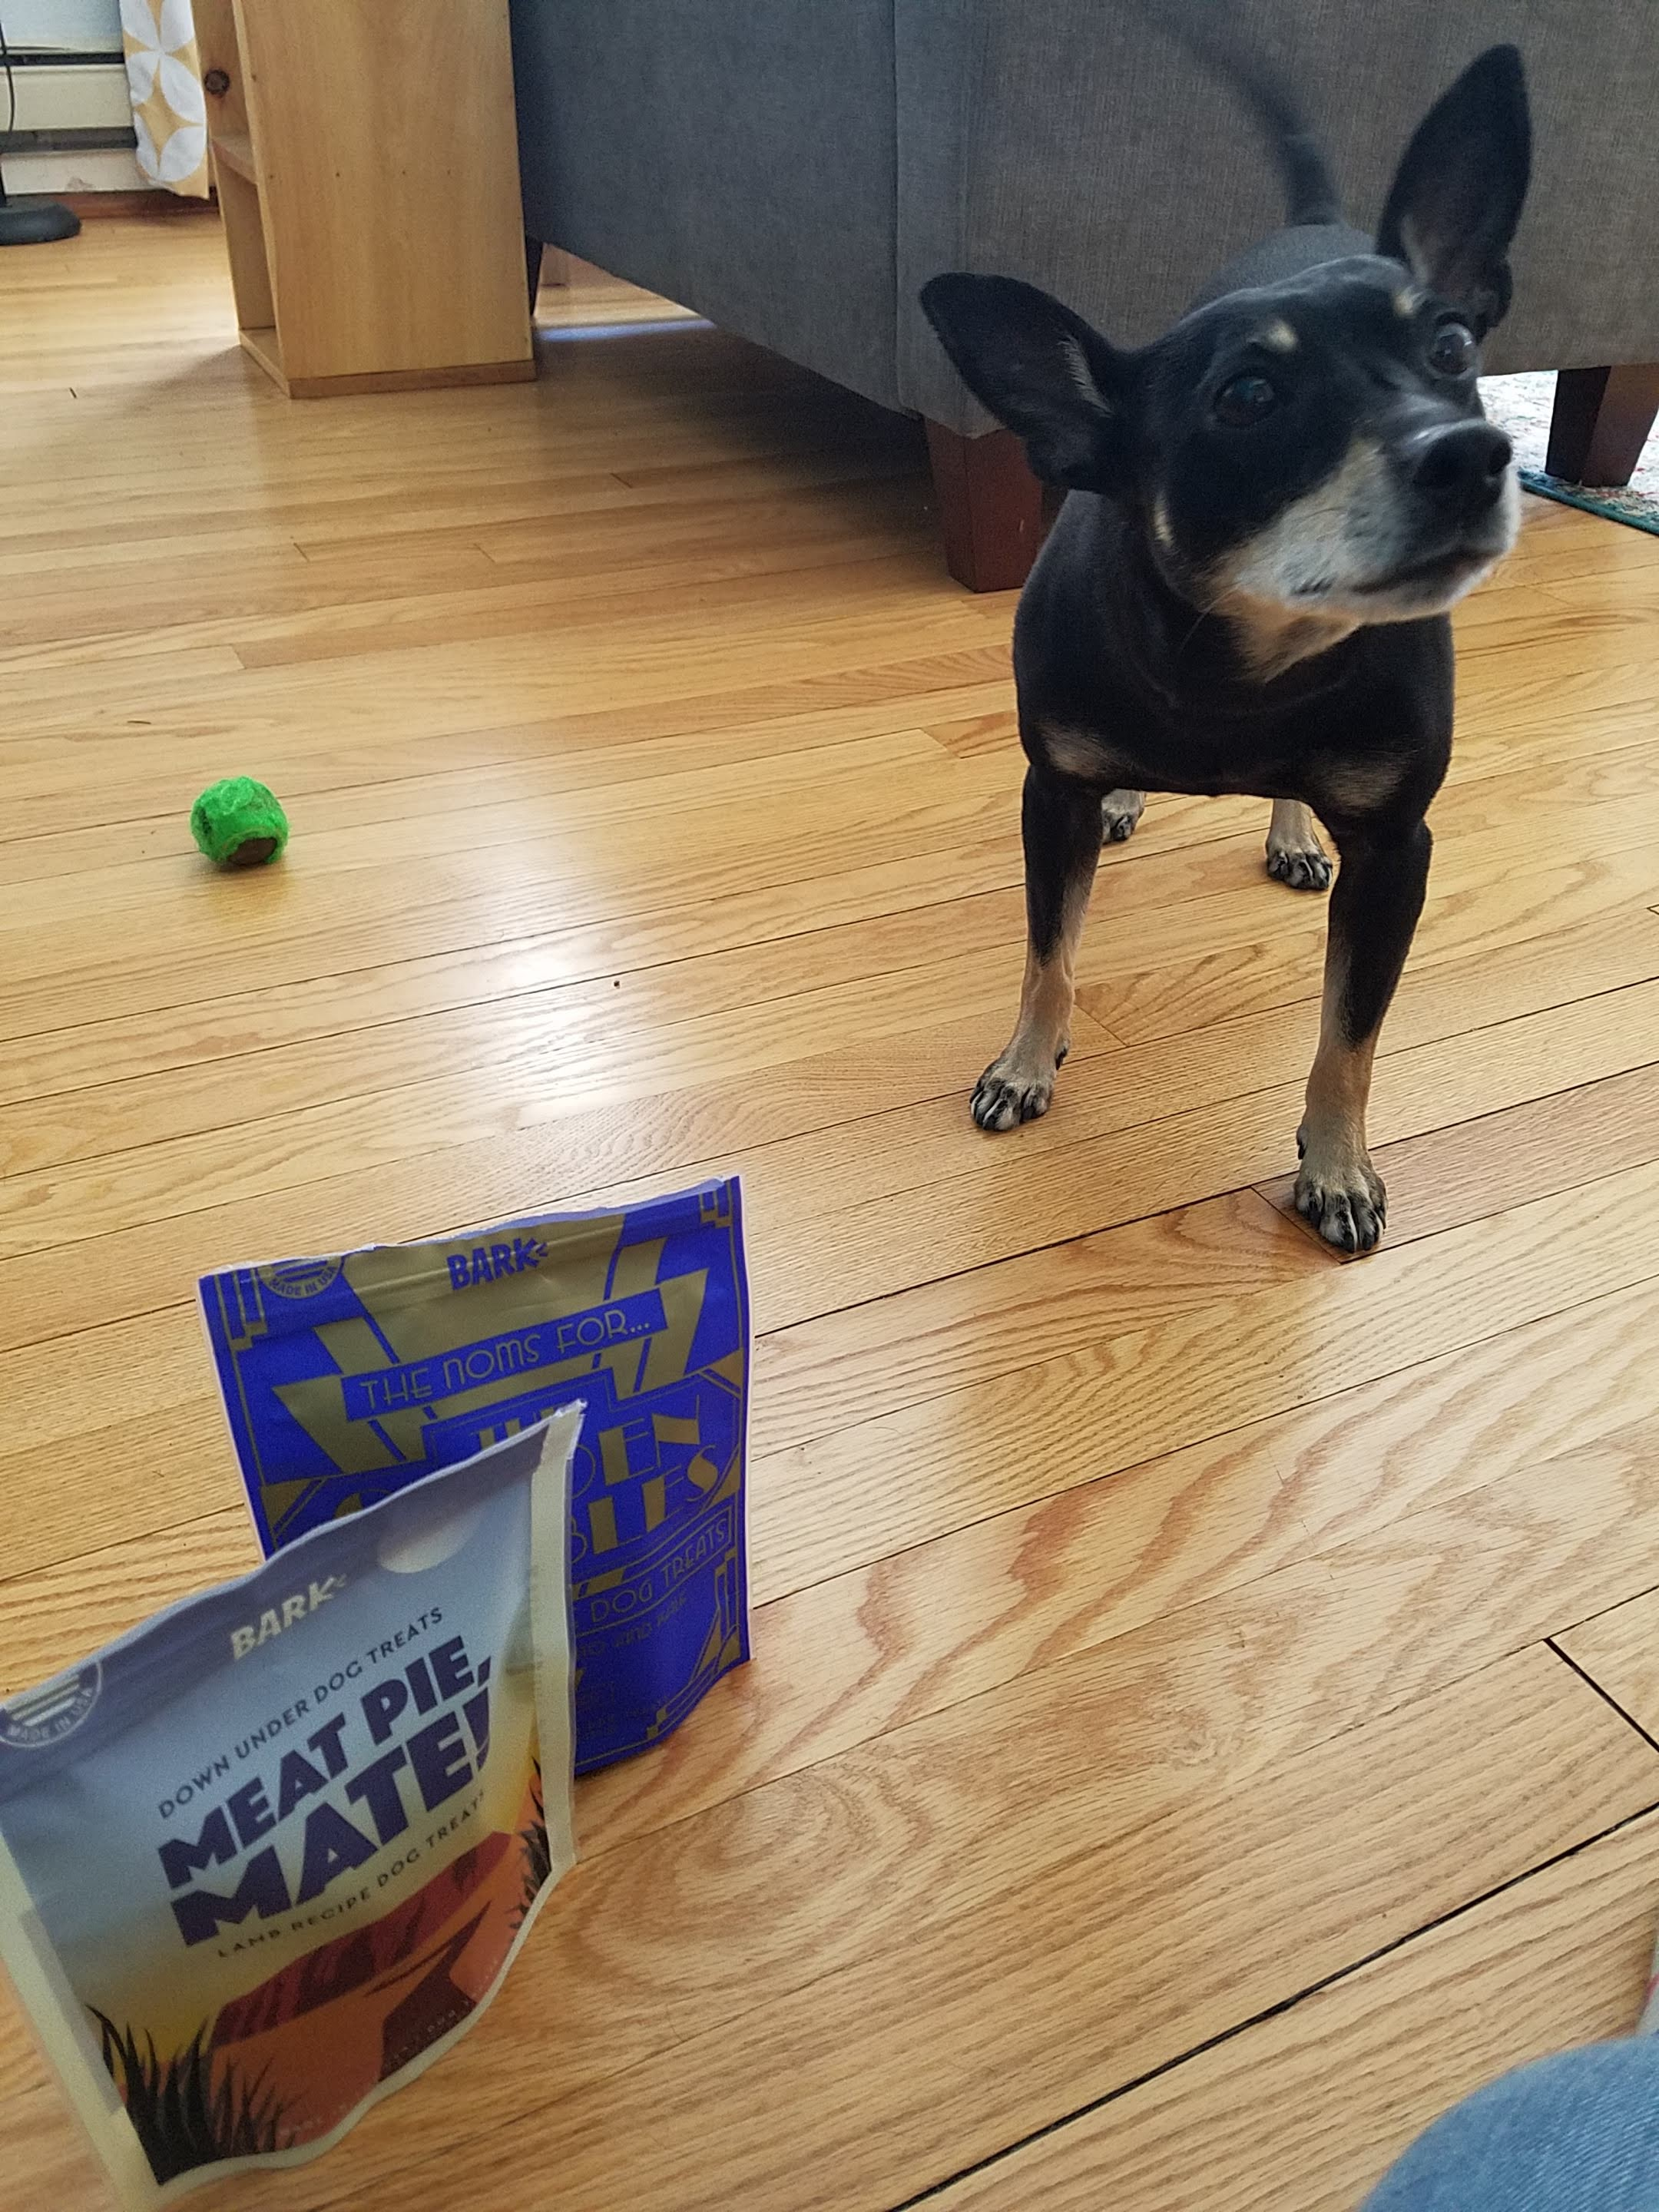
\includegraphics[width=1.5in]{images/cookie_Pepper}
			
			Pepper wants more Barkbox.
		\end{center}
	\end{block}
\end{frame}
\begin{frame}{\fn}
	\begin{statementblock}{Theorem 4.15}
		If $A$ is an $m\times n$ matrix, then the row space and the column space of $A$ have the same dimension.
	\end{statementblock}
	\begin{exercise}
		Convince yourself of this fact by considering the relationship between dimension of row/column spaces and leading 1's in the reduced row echelon form of $A$.
	\end{exercise}
\end{frame}
\begin{frame}{\fn}
	\begin{defn}
		The \emph{rank of a matrix $A$}, denoted $\rank(A)$, is the dimension of the row (or column) space of $A$.
	\end{defn}
	\begin{exa}
		$\rank(I_n)=n$
		
		$\rank(O_{m,n})=0$
	\end{exa}
\end{frame}
\begin{frame}{\fn}
	\begin{exercise}
		Determine
		\[\rank\left(\begin{bmatrix}
		7 & 9 & -1 \\
		1 & -2 & -2 \\
		4 & 0 & -1 \\
		7 & -3 & -2
		\end{bmatrix}\right)\]
	\end{exercise}
\end{frame}
\begin{frame}{\fn}
	\begin{exercise}
		Give examples of matrices such that\begin{enumerate}[label=(\alph*)]
			\item $\rank(A+B)<\rank(A)$ and $\rank(A+B)<\rank(B)$
			\item $\rank(A+B)=\rank(A)$ and $\rank(A+B)=\rank(B)$
			\item $\rank(A+B)>\rank(A)$ and $\rank(A+B)>\rank(B)$
		\end{enumerate}
		Is it possible for $\rank(A+B)<\rank(A)$ and $\rank(A+B)>\rank(B)$?
	\end{exercise}
\end{frame}
\end{document}

